% State space diagram of the latent curve model with structured residuals (vignette lcm-sr).
\documentclass[tikz, border = 6pt]{standalone}
\usepackage{amsmath}
\usepackage{bm}
\usetikzlibrary{arrows.meta, positioning, calc}
\tikzset{
  lat/.style = {circle, draw, thick, minimum size = 13mm, inner sep = 0pt},
  obs/.style = {rectangle, draw, thick, minimum size = 11mm, inner sep = 1pt},
  noise/.style = {circle, draw, minimum size = 9mm, inner sep = 0pt},
  reg/.style = {-{Stealth[length = 2.5mm]}, thick},
  cov/.style = {{Stealth[length = 2mm]}-{Stealth[length = 2mm]}},
  var/.style = {cov, looseness = 5},
  lab/.style = {font = \footnotesize, fill = white, inner sep = 1pt},
  mat/.style = {font = \small, inner sep = 2pt, align = left},
  dots/.style = {font = \Large}
}
\begin{document}
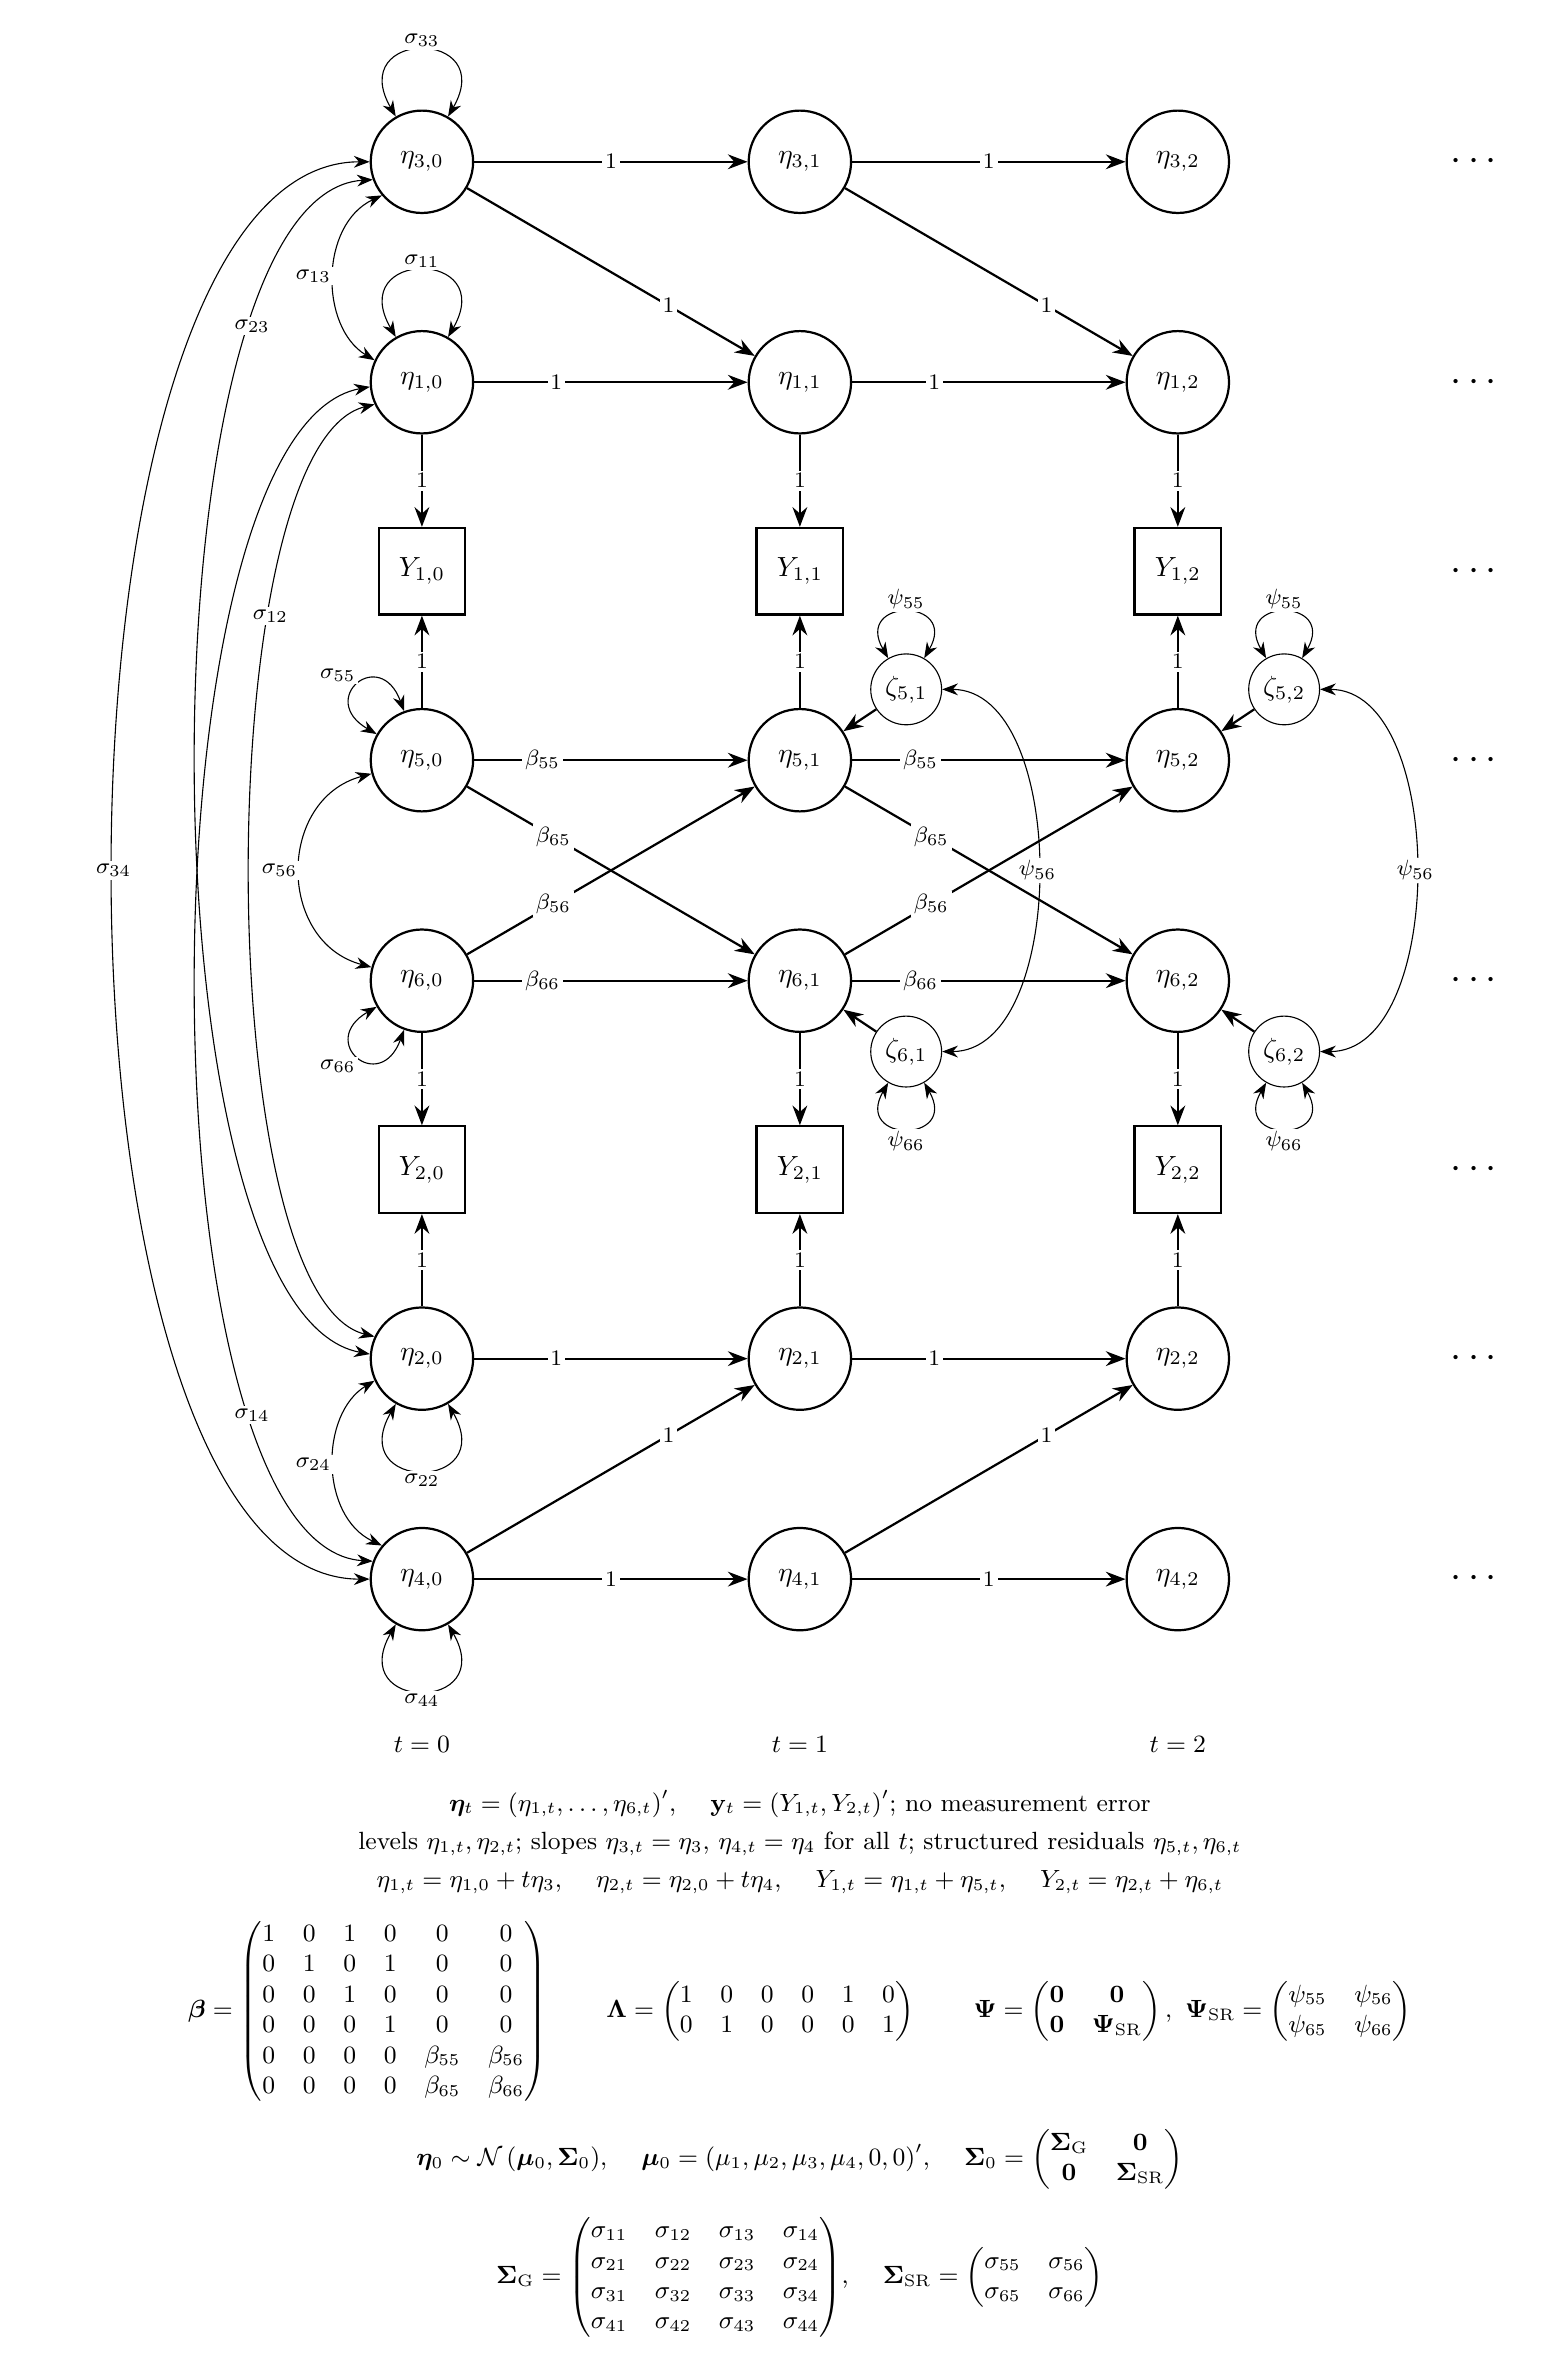
\begin{tikzpicture}
  % occasions
  \foreach \t/\x in {0/0, 1/4.8, 2/9.6} {
    \node[lat] (c\t) at (\x, 9.0) {$\eta_{3, \t}$};
    \node[lat] (a\t) at (\x, 6.2) {$\eta_{1, \t}$};
    \node[obs] (p\t) at (\x, 3.8) {$Y_{1, \t}$};
    \node[lat] (e\t) at (\x, 1.4) {$\eta_{5, \t}$};
    \node[lat] (f\t) at (\x, -1.4) {$\eta_{6, \t}$};
    \node[obs] (q\t) at (\x, -3.8) {$Y_{2, \t}$};
    \node[lat] (b\t) at (\x, -6.2) {$\eta_{2, \t}$};
    \node[lat] (d\t) at (\x, -9.0) {$\eta_{4, \t}$};
    \draw[reg] (a\t) -- node[lab] {1} (p\t);
    \draw[reg] (e\t) -- node[lab] {1} (p\t);
    \draw[reg] (b\t) -- node[lab] {1} (q\t);
    \draw[reg] (f\t) -- node[lab] {1} (q\t);
    \node[font = \small] at (\x, -11.1) {$t = \t$};
  }
  % transitions
  \foreach \s/\t in {0/1, 1/2} {
    % growth part
    \draw[reg] (c\s) -- node[lab, pos = 0.5] {1} (c\t);
    \draw[reg] (d\s) -- node[lab, pos = 0.5] {1} (d\t);
    \draw[reg] (a\s) -- node[lab, pos = 0.3] {1} (a\t);
    \draw[reg] (b\s) -- node[lab, pos = 0.3] {1} (b\t);
    \draw[reg] (c\s) -- node[lab, pos = 0.7] {1} (a\t);
    \draw[reg] (d\s) -- node[lab, pos = 0.7] {1} (b\t);
    % structured residuals
    \draw[reg] (e\s) -- node[lab, pos = 0.25] {$\beta_{55}$} (e\t);
    \draw[reg] (f\s) -- node[lab, pos = 0.25] {$\beta_{66}$} (f\t);
    \draw[reg] (f\s) -- node[lab, pos = 0.3] {$\beta_{56}$} (e\t);
    \draw[reg] (e\s) -- node[lab, pos = 0.3] {$\beta_{65}$} (f\t);
  }
  % process noise (structured residuals only)
  \foreach \t/\x in {1/4.8, 2/9.6} {
    \node[noise] (z5\t) at (\x + 1.35, 2.3) {$\zeta_{5, \t}$};
    \node[noise] (z6\t) at (\x + 1.35, -2.3) {$\zeta_{6, \t}$};
    \draw[reg] (z5\t) -- (e\t);
    \draw[reg] (z6\t) -- (f\t);
    \draw[var] (z5\t.60) to[out = 60, in = 120]
      node[lab, above] {$\psi_{55}$} (z5\t.120);
    \draw[var] (z6\t.240) to[out = 240, in = 300]
      node[lab, below] {$\psi_{66}$} (z6\t.300);
    \draw[cov] (z5\t.east) to[out = 0, in = 0, looseness = 0.9]
      node[lab] {$\psi_{56}$} (z6\t.east);
  }
  \foreach \r in {9.0, 6.2, 3.8, 1.4, -1.4, -3.8, -6.2, -9.0} {
    \node[dots] at (13.4, \r) {$\cdots$};
  }
  % initial condition: variances
  \draw[var] (c0.60) to[out = 60, in = 120]
    node[lab, above] {$\sigma_{33}$} (c0.120);
  \draw[var] (a0.60) to[out = 60, in = 120]
    node[lab, above] {$\sigma_{11}$} (a0.120);
  \draw[var] (b0.240) to[out = 240, in = 300]
    node[lab, below] {$\sigma_{22}$} (b0.300);
  \draw[var] (d0.240) to[out = 240, in = 300]
    node[lab, below] {$\sigma_{44}$} (d0.300);
  \draw[var] (e0.110) to[out = 110, in = 150]
    node[lab, above left] {$\sigma_{55}$} (e0.150);
  \draw[var] (f0.210) to[out = 210, in = 250]
    node[lab, below left] {$\sigma_{66}$} (f0.250);
  % initial condition: covariances
  \draw[cov] (e0.195) to[out = 195, in = 165, looseness = 1.3]
    node[lab, left] {$\sigma_{56}$} (f0.165);
  \draw[cov] (c0.220) .. controls (-1.3, 8.2) and (-1.3, 6.9) ..
    node[lab, left] {$\sigma_{13}$} (a0.155);
  \draw[cov] (d0.140) .. controls (-1.3, -8.2) and (-1.3, -6.9) ..
    node[lab, left] {$\sigma_{24}$} (b0.205);
  \draw[cov] (a0.205) .. controls (-2.7, 5.4) and (-2.7, -5.4) ..
    node[lab, pos = 0.3] {$\sigma_{12}$} (b0.155);
  \draw[cov] (c0.200) .. controls (-3.6, 8.6) and (-3.6, -5.6) ..
    node[lab, pos = 0.22] {$\sigma_{23}$} (b0.175);
  \draw[cov] (d0.160) .. controls (-3.6, -8.6) and (-3.6, 5.6) ..
    node[lab, pos = 0.22] {$\sigma_{14}$} (a0.185);
  \draw[cov] (c0.180) .. controls (-5.0, 9.0) and (-5.0, -9.0) ..
    node[lab] {$\sigma_{34}$} (d0.180);
  % matrices
  \node[mat, align = center, below] at (4.8, -11.6) {%
    $\bm{\eta}_{t} = \left( \eta_{1, t}, \ldots, \eta_{6, t}
      \right)^{\prime}$, \quad
    $\mathbf{y}_{t} = \left( Y_{1, t}, Y_{2, t} \right)^{\prime}$;
    no measurement error \\[1mm]
    levels $\eta_{1, t}, \eta_{2, t}$; slopes $\eta_{3, t} = \eta_{3}$,
    $\eta_{4, t} = \eta_{4}$ for all $t$;
    structured residuals $\eta_{5, t}, \eta_{6, t}$ \\[1mm]
    $\eta_{1, t} = \eta_{1, 0} + t \eta_{3}$, \quad
    $\eta_{2, t} = \eta_{2, 0} + t \eta_{4}$, \quad
    $Y_{1, t} = \eta_{1, t} + \eta_{5, t}$, \quad
    $Y_{2, t} = \eta_{2, t} + \eta_{6, t}$ \\[3mm]
    $\bm{\beta} = \begin{pmatrix}
      1 & 0 & 1 & 0 & 0 & 0 \\ 0 & 1 & 0 & 1 & 0 & 0 \\
      0 & 0 & 1 & 0 & 0 & 0 \\ 0 & 0 & 0 & 1 & 0 & 0 \\
      0 & 0 & 0 & 0 & \beta_{55} & \beta_{56} \\
      0 & 0 & 0 & 0 & \beta_{65} & \beta_{66}
    \end{pmatrix}$
    \qquad $\bm{\Lambda} = \begin{pmatrix}
      1 & 0 & 0 & 0 & 1 & 0 \\ 0 & 1 & 0 & 0 & 0 & 1
    \end{pmatrix}$
    \qquad $\bm{\Psi} = \begin{pmatrix}
      \mathbf{0} & \mathbf{0} \\ \mathbf{0} & \bm{\Psi}_{\mathrm{SR}}
    \end{pmatrix}, \ \bm{\Psi}_{\mathrm{SR}} = \begin{pmatrix}
      \psi_{55} & \psi_{56} \\ \psi_{65} & \psi_{66}
    \end{pmatrix}$ \\[3mm]
    $\bm{\eta}_{0} \sim \mathcal{N} \left( \bm{\mu}_{0},
      \bm{\Sigma}_{0} \right)$, \quad
    $\bm{\mu}_{0} = \left( \mu_{1}, \mu_{2}, \mu_{3}, \mu_{4}, 0, 0
      \right)^{\prime}$, \quad
    $\bm{\Sigma}_{0} = \begin{pmatrix}
      \bm{\Sigma}_{\mathrm{G}} & \mathbf{0} \\
      \mathbf{0} & \bm{\Sigma}_{\mathrm{SR}}
    \end{pmatrix}$ \\[3mm]
    $\bm{\Sigma}_{\mathrm{G}} = \begin{pmatrix}
      \sigma_{11} & \sigma_{12} & \sigma_{13} & \sigma_{14} \\
      \sigma_{21} & \sigma_{22} & \sigma_{23} & \sigma_{24} \\
      \sigma_{31} & \sigma_{32} & \sigma_{33} & \sigma_{34} \\
      \sigma_{41} & \sigma_{42} & \sigma_{43} & \sigma_{44}
    \end{pmatrix}$, \quad
    $\bm{\Sigma}_{\mathrm{SR}} = \begin{pmatrix}
      \sigma_{55} & \sigma_{56} \\ \sigma_{65} & \sigma_{66}
    \end{pmatrix}$};
\end{tikzpicture}
\end{document}